\documentclass{article}
\usepackage[utf8]{inputenc}
\usepackage{amssymb}
\usepackage{amsmath}
\usepackage{cancel}
\usepackage{graphicx}
\graphicspath{{Images/}}
\usepackage{chngcntr}
\setlength{\oddsidemargin}{0in}
\setlength{\textwidth}{6.5in}
\setlength{\topmargin}{-.55in}
\setlength{\textheight}{9in}
\pagestyle{empty}
\counterwithin{equation}{section}



\title{Problem Set 4 (Astrophysics)}
\author{Michael Nameika}
\date{February 2022}

\begin{document}

\maketitle

\section{Problem 1}
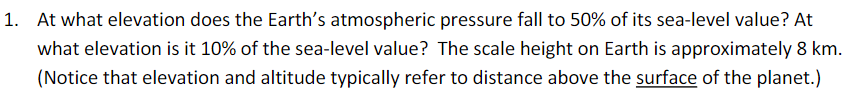
\includegraphics[scale = 0.8]{probset4prob1.PNG}

Recall the equation for the pressure at a height $h$ above the surface:
\begin{equation}
    P(h) = P_0e^{-\frac{h}{H}}
\end{equation}
Where $P_0$ is the pressure at the surface of the planet, $h$ is the height in kilometers from the surface, and $H$ is defined as
\[H = \frac{kT}{g\mu m_p}\]
For Earth, we are given that $H \approx 8  \:km$.
\newline
We first wish to find where the atmospheric pressure is one half that at sea level. To find this, we can set equation (1.1) equal to $\frac{P_0}{2}$ and solve for $h$:
\[\frac{P_0}{2} = P_0 e^{-h/(8 \: km)}\]
\[\ln{(2)} (8 \: km) = h\]
\[h \approx 5.545 \: km\]
That is, at an elevation of approximately $5.5$ kilometers, the atmospheric pressure will be half that at sea level.

Now we wish to find the elevation when the atmospheric pressure is one tenth that at sea level. Following the same process as above, set (1.1) equal to $\frac{P_0}{10}$ and solve for $h$:
\[\frac{P_0}{10} = P_0 e^{-h/(8 \: km)}\]
\[\ln{(10)} (8 \: km) = h\]
\[h \approx 18.42 \: km\]
That is, at an elevation of approximately $18.42$ kilometers, the atmospheric pressure will be one tenth that at sea level.

\section{Problem 2}
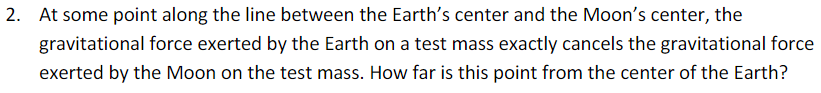
\includegraphics[scale = 0.8]{probset4prob2.PNG}

We wish to find when the gravitational force between the Earth and the Moon are equal when colinear between their centers. Assume that this equilibrium occurs at a distance of $r_1$ from the Moon and a distance of $r_2$ from the Earth. By Newton's law of gravitation, we know that the force of gravity on some test mass by the Earth is given by
\[F_{Earth} = \frac{GM_{Earth}m}{r_2^2}\]
and the force of gravity from the Moon:
\[F_{Moon} = \frac{GM_{Moon}m}{r_1^2}\]
Notice that $r_1 + r_2 = $distance between Earth and Moon $ = 3.84 \times 10^5 \: km$.

Now since we want to find $r_1$ and $r_2$ such that the gravitational force from the Moon balances that of the Earth, let's set the two values equal to one another:
\[\frac{GM_{Earth}m}{r_2^2} = \frac{GM_{Moon}m}{r_1^2}\]
Solving, we find
\[\frac{r_1}{r_2} = \sqrt{\frac{M_{Moon}}{M_{Earth}}}\]
And using our relationship between $r_1$ and $r_2$, we find
\[\frac{3.84 \times 10^5 \: km - r_2}{r_2} = \sqrt{\frac{M_{Moon}}{M_{Earth}}}\]
Solving, we find
\[r_2 = 3.46 \times 10^{5} \: km\]
That is, at a distance of approximately $3.46 \times 10^5 \: km$ from the center of the Earth, the Moon's gravitational force will balance out Earth's gravitational force.


\section{Problem 3}
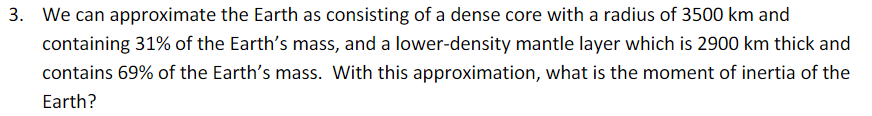
\includegraphics[scale = 0.8]{probset4prob3.PNG}

Let's split this problem up into two: we will find the moment of inertia of the core, then the moment of inertia of the rest of the planet. Finding the moment of inertia of the rest of the planet will boil down to finding the moment of inertia of a solid sphere with a smaller sphere cut out of the center. Recall that the inertia of a sphere is given by
\[I_{Sphere} = \frac{2}{5}(MR^2)\]
So we can use this to find the moment of inertia of the core:
\[I_{Core} = \frac{2}{5}(0.31*5.974 \times 10^{24} \:kg)(3.5 \times 10^6 \: m)^2\]
\[ \approx 9.075 \times 10^{36} \:kg \:m^2\]
Now we wish to find the moment of inertia of the rest of the planet. Well, to do this, recall the formula for moment of inertia:
\[I = \int{\int{\int_Q{ \rho (x,y) |\textbf{r}|_2^2 dV}}}\]
Where $Q$ is the body whose inertia we're measuring, $\textbf{r}$ is the vector perpendicular to the rotation axis to the boundary of the body, and $\rho$ is the density function of the body. In our problem, the density is assumed to be uniform, so we can pull that term out of the integral. Notice that $\textbf{r} = r\sin{(\phi)}$ where $\phi$ is the angle measured from the positive $z$ axis. Now, to find the moment of inertia:
\[I_{Mantle} = \frac{M}{\frac{4}{3}\pi (R_2^3 - R_1^3)}\int_0^{\phi}\int_0^{2\pi}\int_{R_1}^{R_2}r^4 \sin^3(\phi) dr d\theta d\phi\]
where $R_1 = 3500 \:km$, $R_2 = 6400 \:km$, and $\theta$ is the azimuthal angle. Solving this integral, we get the following:
\[I_{Mantle} = \frac{2M(R_2^5 - R_1^5)}{5(R_2^3 - R_1^3)}\]
\[ = \frac{2(0.69 * 5.974 \times 10^{24} \:kg)((6.4 \times 10^{6} \: m)^5 - (3.5 \times 10^6 \: m)^5)}{5((6.4 \times 10^6 \:m)^3 - (3.5 \times 10^6 \:m)^3)}\]
\[\approx 7.68 \times 10^{37} \:kg \:m^2\]
Now to find the total moment of inertia, let's add these two quantities together:
\[I_{Total} = I_{Core} + I_{Mantle} \approx 9.075 \times 10^{36} \:kg \:m^2 + 7.68 \times 10^{37} \:kg \:m^2\]
\[ = 8.59 \times 10^{37} \:kg \:m^2\]
So the moment of inertia of the Earth is approximately $8.59 \times 10^{37} \:kg \:m^2$.





\section{Problem 4}
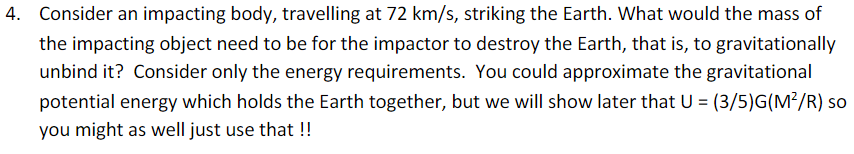
\includegraphics[scale = 0.8]{probset4prob4.PNG}

We are given that the gravitational potential energy holding the Earth together is  
\[U = (\frac{3}{5})(\frac{GM^2}{R})\]
Assume that the Earth will break apart when the mass of the impacting body is such that its kinetic energy is greater than or equal to the gravitational potential energy holding the Earth together. That is, we must solve
\[\frac{1}{2}m_{IB}(72 \: km/s)^2 = \frac{3}{5}(\frac{GM^2}{R})\]
for $m_{IB}$, the mass of the impacting body. Solving, we find
\[m_{IB} = \frac{6}{5}(\frac{GM^2}{R(72 \: km/s)^2})\]
\[ = \frac{6}{5}(\frac{(6.67 \times 10^{-11} \: s^{-2} \: kg^{-1} \: m^3)(5.974 \times 10^{24} \: kg)^2}{(6.378 \times 10^{6} \: m)(7.2 \times 10^4 \: m)^2})\]
\[ \approx 8.64 \times 10^{22} \: kg\]
So an impacting body traveling at $72 \: km/s$ would have to have a mass of at least $8.64 \times 10^{24} \: kg$ to break apart the Earth with a direct impact.

\section{Problem 5}
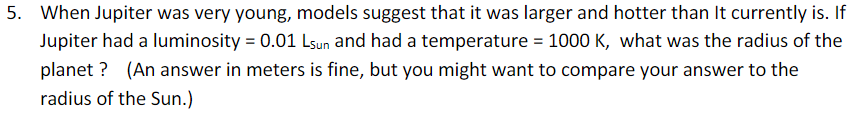
\includegraphics[scale = 0.8]{probset4prob5.PNG}

Recall that the luminosity is related to the radius and temperature of a blackbody by the following:
\[L = 4\pi R^2 \sigma T^4\]
where $\sigma = 5.67 \times 10^{-8} \frac{W}{m^2 k^4}$. Solving the above equation for $R$, we find the following:
\[R = \sqrt{\frac{L}{4 \pi \sigma T^4}}\]

We are given that the luminosity is $0.01 L_{Sun}$ and the temperature is $1000 \:K$. Plugging these values into the equation above, we will find that the radius of Jupiter is
\[R_{Jupiter} = \sqrt{\frac{0.01*3.9 \times 10^{26}W}{4\pi (5.67 \times 10^{-8} \frac{W}{m^2 k^4})(1000 \:K)^4}}\]
\[\approx 2.34 \times 10^9 \:m\]
From the table at the beginning of the assignment, we see that the radius of the sun is $6.955 \times 10^{8} \:m$. Expressing Jupiter's radius in terms of solar radii, we find
\[R_{Jupiter} \approx 3.36 \:R_{Solar}\]
So if Jupiter had a luminosity of $0.01 \:L_{Sun}$ and a temperature of $1000 \:K$, Jupiter would have had to have a radius $3.36$ times that of the Sun! 


\end{document}
